\documentclass{article}
\usepackage{amsmath}
\usepackage{tikz}
\usetikzlibrary{intersections}

\begin{document}

\begin{figure}[h]
    \centering
    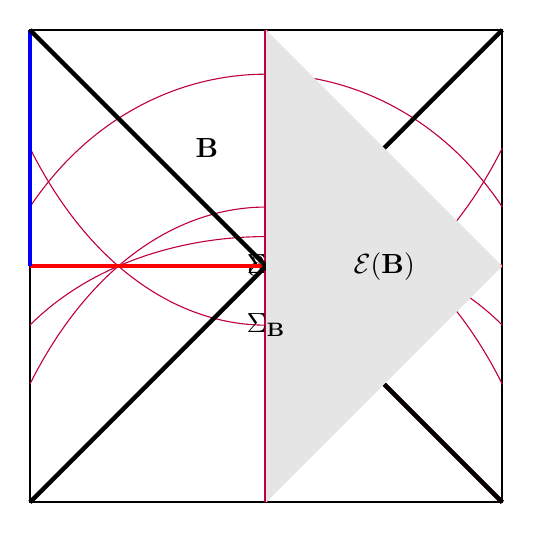
\begin{tikzpicture}[scale=1.5]
        % Draw the square boundary
        \draw[thick] (0,0) -- (4,0) -- (4,4) -- (0,4) -- cycle;
        
        % Draw the thick purple line (Cauchy surface at t=0)
        \draw[ultra thick, color=purple] (0,2) -- (4,2);
        \node at (2,2) {$\Sigma_P$};
        
        % Draw the thick purple line (entangling surface)
        \draw[ultra thick, color=purple] (2,0) -- (2,4);
        \node at (2,2) {$\partial \Sigma$};
        
        % Draw the thick purple line (Cauchy surface at t=0)
        \draw[ultra thick, color=purple] (2,2) -- (4,0);
        \node at (3.5,2) {$\Sigma_{P'}$};
        
        % Draw the thin purple lines (Cauchy surfaces at t ≠ 0)
        \draw[color=purple, name path=A] (0,1) .. controls (1,3) and (3,3) .. (4,1);
        \draw[color=purple, name path=B] (0,3) .. controls (1,1) and (3,1) .. (4,3);
        \draw[color=purple, name path=C] (0,2.5) .. controls (1,4) and (3,4) .. (4,2.5);
        \draw[color=purple, name path=D] (0,1.5) .. controls (1,2.5) and (3,2.5) .. (4,1.5);
        
        % Draw the red line (time band boundary)
        \draw[ultra thick, color=red] (0,2) -- (4,2);
        
        % Draw the blue line (time band boundary)
        \draw[ultra thick, color=blue] (0,2) -- (0,4);
        
        % Draw the black lines (diagonals)
        \draw[ultra thick] (0,0) -- (4,4);
        \draw[ultra thick] (0,4) -- (4,0);
        
        % Draw the grey triangle wedge
        \fill[gray!20] (2,0) -- (2,4) -- (4,2) -- cycle;
        \node at (3,2) {$\mathcal{E}(\mathbf{B})$};
        
        % Draw the boldface B
        \node at (1.5,3) {$\mathbf{B}$};
        
        % Draw the text for the entangling surface
        \node at (2,1.5) {$\Sigma_{\mathbf{B}}$};
    \end{tikzpicture}
    \caption{The thick purple line ($\Sigma_{t=0}=\Sigma_{P}\cup \partial \Sigma \cup \Sigma_{P'}$) denotes a Cauchy surface at $t=0$ and other purple curves describe Cauchy surfaces at $t\neq 0$. $\partial \Sigma$ is for the entangling surface between the left and the right patch. The boldface ${\bf B}$ denotes the time band $[\tau_{1}, \tau_{0}]$ and the grey triangle wedge, ${\cal E}({\bf B})$, represents a timelike envelope of the time band ${\bf B}$, while $\Sigma_{\bf B}$ does the entangling surface for the wedge ${\cal E}({\bf B})$.}
    \label{fig:cauchy_surface}
\end{figure}

\end{document}